%%
% Please see https://bitbucket.org/rivanvx/beamer/wiki/Home for obtaining beamer.
%%
%\documentclass[11pt,aspectratio=169]{beamer}
%\documentclass[11pt,aspectratio=169,xcolor={dvipsnames}]{beamer}

\documentclass[11pt,aspectratio=169,xcolor={dvipsnames},hyperref={pdftex,pdfpagemode=UseNone,hidelinks,pdfdisplaydoctitle=true},usepdftitle=false]{beamer}
\usepackage{presentation}


\title{Lecture 10: Real Rigidities}
\author{Juan Herre\~{n}o\\UCSD}
\date{2026}

% Enter presentation title to populate PDF metadata:
\newcommand{\Cov}{\text{Cov}_\lambda}
\newcommand{\El}{\mathbb{E}_\lambda}
\newcommand{\mm}{\text{{\fontfamily{qzc}\selectfont m}}}
\usepackage{cancel}
\usepackage{booktabs}
\begin{document}

\maketitle

\begin{frame}{Terminology}
\begin{itemize}
\item Three distinct but similarly worded terms
\begin{itemize}
\item Nominal stickiness: It is difficult, or costly to adjust individual \textbf{nominal prices}
\item Real rigidities: responsiveness of \textbf{real} prices to changes in \textbf{real} economic activity
\item Nominal rigidities: Reactions of \textbf{real} economic activity to changes in \textbf{nominal} variables
\end{itemize}
\item Result I: Nominal stickiness + real rigidities $\rightarrow$ large nominal rigidities
\item Result II: Nominal stickiness + no real rigidities $\rightarrow$ small nominal rigidities
\item Result III: No nominal stickiness + real rigidities $\rightarrow$ no nominal rigidities
\end{itemize}
\end{frame}

\begin{frame}{Economics}
\begin{itemize}
\item Costs of price adjustment are certainly present in the data:
\begin{itemize}
\item Physical costs of changing prices
\item Organizational costs of deciding new prices
\item Informational costs of doing so
\end{itemize}
\item However, these costs sound rather ``small''.
\item Can ``small'' price adjustment costs generate large aggregate fluctuations?
\item Can the price of asparagus explain the Great Depression?
\end{itemize}
\end{frame}

\begin{frame}{Small menu costs and large inaction}
\begin{itemize}
\item The economy is characterized by a symmetric steady state
\begin{align*}
P_{it} = P_t 
\end{align*}
\item In steady state, the money supply satisfies:
\begin{align}
M_t = P_t Y_t = 1.
\end{align}
\item Just a normalization, remember that in the absence of nominal rigidities, nominal variables do not matter.
\end{itemize}
\end{frame}

\begin{frame}{Small menu costs and large inaction}
Assume a profit function exclusive of menu costs of the form 
\begin{align}
X_{it} = X\left(p_{it} - p_t, m_t\right)
\end{align}
\begin{itemize}
\item In words: The demand curve depends on $Y$ and on relative prices. I will not impose CES.
\item Profits are equal to $Profits_{it} = X_{it} - D_{it} k$
\item $D_{it}$ is a dummy that takes the value of 1 if the firm resets its price
\item $k$ is a menu cost
\end{itemize}
Price flexibility is a Nash equilibrium if whenever every firm is fully adjusting, firm $i$ decides to fully adjust as well. (in that case, adjusting your price is a best response)
\end{frame}

\begin{frame}{Small menu costs and large inaction}
Remember: maintained assumption that every firm adjusts
\begin{align}
X_{it} = X\left(p_{it} - p_t, m_t\right) 
\end{align}
\begin{itemize}
\item If firm $i$ adjusts, then 
\begin{align*}
X_{it} =  X\left(0, m_t\right)
\end{align*}
\item If firm $i$ does not adjust, then
\begin{align*}
X_{it} =  X\left(p^*_{it} - p_t, m_t\right)
\end{align*}
\item The firm will not adjust its price iff
\begin{align*}
X\left(0, m_t\right) -  X\left(p^*_{it} - p_t, m_t\right) \leq k
\end{align*}
\end{itemize}
\end{frame}

\begin{frame}{Small menu costs and large inaction}
\begin{itemize}
\item Let me do a second-order approximation of $ X\left(p^*_{it} - p_t, m_t\right) $ around $p^*_{it} = p_t$
\begin{align*}
 X\left(p^*_{it} - p_t, m_t\right) \approx X\left(0, m_t\right) + X_p\left(0, m_t\right)(p^*_{it} - p_t) + \frac{1}{2} X_{pp}\left(0, m_t\right) (p^*_{it} - p_t)^2
\end{align*}
\item Use the result in the last slide
\begin{align*}
-X_p\left(0, m_t\right)(p^*_{it} - p_t) - \frac{1}{2} X_{pp}\left(0, m_t\right) (p^*_{it} - p_t)^2 \leq k
\end{align*}
\item Notice that firm optimality in the steady state implies that $X_p(0,.) = 0$.
\item Therefore
\begin{align*}
 - \frac{1}{2} X_{pp}\left(0, m_t\right) (p^*_{it} - p_t)^2 \leq k
\end{align*}
\item Firms will not adjust if this inequality is satisfied
\end{itemize}
\end{frame}

\begin{frame}{Small menu costs and large inaction}
Price flexibility is not a Nash equilibrium iff
\begin{align*}
 - \frac{1}{2} X_{pp}\left(0, m_t\right) (p^*_{it} - p_t)^2 \leq k
\end{align*}
\begin{itemize}
\item There exists a small enough price change (these are log changes)
\item so that second-order menu costs induce price rigidity
\end{itemize}
This was Mankiw (1985), by the way.
\end{frame}


\begin{frame}{Small menu costs and large inaction}




\tikzset{every picture/.style={line width=0.75pt}} %set default line width to 0.75pt        


\tikzset{every picture/.style={line width=0.75pt}} %set default line width to 0.75pt        

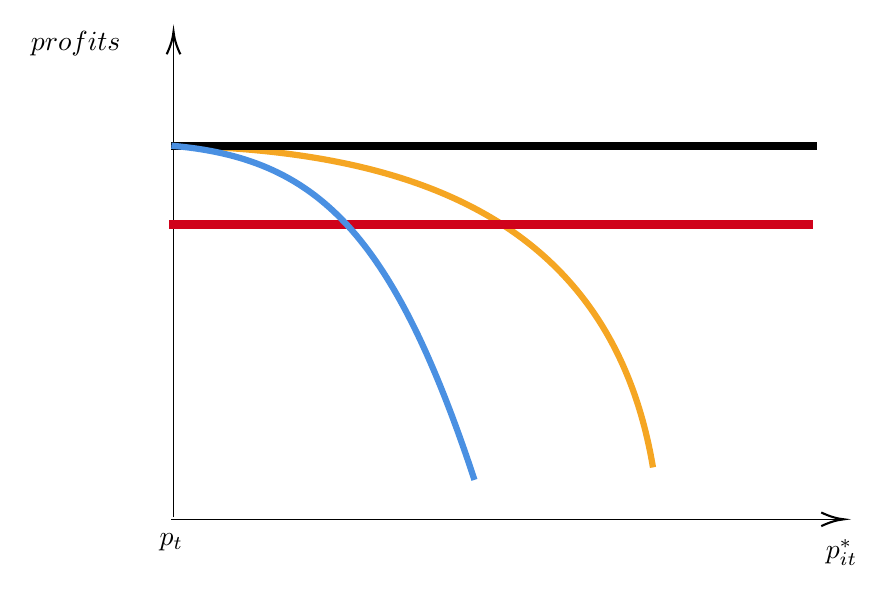
\begin{tikzpicture}[x=0.75pt,y=0.75pt,yscale=-1,xscale=1]
%uncomment if require: \path (0,300); %set diagram left start at 0, and has height of 300

%Curve Lines [id:da23518737631499798] 
\draw [color={rgb, 255:red, 245; green, 166; blue, 35 }  ,draw opacity=1 ][line width=2.25]    (200,72) .. controls (307,74) and (411,102) .. (432,227) ;
%Straight Lines [id:da482028855555948] 
\draw    (200,252) -- (522,252) ;
\draw [shift={(524,252)}, rotate = 180] [color={rgb, 255:red, 0; green, 0; blue, 0 }  ][line width=0.75]    (10.93,-3.29) .. controls (6.95,-1.4) and (3.31,-0.3) .. (0,0) .. controls (3.31,0.3) and (6.95,1.4) .. (10.93,3.29)   ;
%Straight Lines [id:da9885451468915929] 
\draw    (201,251) -- (201,19) ;
\draw [shift={(201,17)}, rotate = 90] [color={rgb, 255:red, 0; green, 0; blue, 0 }  ][line width=0.75]    (10.93,-3.29) .. controls (6.95,-1.4) and (3.31,-0.3) .. (0,0) .. controls (3.31,0.3) and (6.95,1.4) .. (10.93,3.29)   ;
%Straight Lines [id:da5966574333422879] 
\draw [line width=3]    (200,72) -- (511,72) ;
%Straight Lines [id:da5282207930711846] 
\draw [color={rgb, 255:red, 208; green, 2; blue, 27 }  ,draw opacity=1 ][line width=3]    (199,110) -- (509,110) ;
%Curve Lines [id:da12337381432829042] 
\draw [color={rgb, 255:red, 74; green, 144; blue, 226 }  ,draw opacity=1 ][line width=2.25]    (200,72) .. controls (269,78) and (306,112) .. (346,233) ;

% Text Node
\draw (514,260.4) node [anchor=north west][inner sep=0.75pt]    {$p{_{it}^{*}}$};
% Text Node
\draw (131,15.4) node [anchor=north west][inner sep=0.75pt]    {$profits$};
% Text Node
\draw (193,257.4) node [anchor=north west][inner sep=0.75pt]    {$p_{t}$};


\end{tikzpicture}\\
Note: The first derivative of the profit funciton at $p^*_{it} = p_t$ is zero. The curvature of the profit function determines the range of inaction
\end{frame}


\begin{frame}{Small menu costs and large inaction}
Conclusion
\begin{itemize}
\item The losses from price deviations are second order
\item Therefore, small menu costs can rule out price flexibility.
\end{itemize}
\end{frame}

\begin{frame}{Real Rigiditiies}
Question: Is an equilibrium where all prices are fixed a Nash Equilibrium?
\begin{itemize}
\item Again, a best response idea: If no one is adjusting, do I want to adjust?
\item Note: the premise implies that nominal price adjustment (by firm $i$) is a real price adjustment (since the price index is fixed).
\item Note: The premise implies that the reaction of real prices is to real aggregate demand (since the price index is fixed).
\item Therefore, real rigidities are about the response of real prices to real aggregate demand.
\end{itemize}
\end{frame}


\begin{frame}{Real Rigiditiies}
\begin{itemize}
\item Consider shocks to nominal demand
\item Profits without any shock are $X(0,0)$.
\item Profits with a shock and without adjustment are $X(0,m_t)$.
\item Profits with a shock and own adjustment are $X(p^*_{it}(m_t) - p_t,m_t)$
\item Therefore, price rigidity is a Nash equilibrium if
$$X(p^*_{it}(m_t) - p_t,m_t) - X(0,m_t) \leq k$$
\end{itemize}
\end{frame}


\begin{frame}{Real Rigiditiies}
\begin{itemize}
\item Optimality requires
$$X_p(p^*_{it}(m_t) - p_t,m_t)  = 0$$
\item Take derivatives
$$X_{pp} \frac{dp^*_{it}(m_t)}{dm_t} + X_{pm} = 0$$
\item Therefore
$$\frac{dp^*_{it}(m_t)}{dm_t} = -\frac{X_{pm}}{X_{pp}} $$
\end{itemize}
This is our definition of real rigidities. How real prices change after changes in real demand. Call this $\rho$, and say there are a lot of real rigidities if $\rho$ is small.
\end{frame}

\begin{frame}{Real Rigidities}
$$X(p^*_{it}(m_t) - p_t,m_t) - X(0,m_t) \leq k$$
\begin{itemize}
\item Take a second-order approximation
\item And use $\frac{dp^*_{it}(m_t)}{dm_t} = -\frac{X_{pm}}{X_{pp}} $
\item You will find
$$ X(p^*_{it}(m_t) - p_t,m_t) - X(0,m_t) \approx - \frac{X_{pm}^2}{2 X_{pp}} m_t^2$$
\item So Price rigidity is an equilibrium as long as
$$ X(p^*_{it}(m_t) - p_t,m_t) - X(0,m_t) \approx - \frac{X_{pm}^2}{2 X_{pp}} m_t^2 \leq k$$
\item Solve for the absolute value shock  $m_t$ where price rigidity is a Nash equilibrium
$$m^* = \left(\frac{2 k}{\rho X_{pm}}\right)$$
\end{itemize}
\end{frame}



\begin{frame}{Real Rigidities}
$$m^* = \left(\frac{2 k}{\rho X_{pm}}\right)$$
\begin{itemize}
\item Note: If there are no price rigidities ($k = 0$), nominal rigidities are zero.
\item Note: If real rigidities increase ($\rho$ smaller), nominal rigidities increase.
\item Note: These results are very generic
\end{itemize}
This was Ball and Romer (1990), by the way
\end{frame}

\begin{frame}{Real Rigidities in the NK Model}
\begin{itemize}
\item Back of the envelope calculation.
\begin{align*}
\pi_t = \beta \mathbb{E}_t \pi_{t+1} + \frac{(1-\beta \lambda)(1-\theta)}{\lambda} (\gamma + \varphi) \tilde{y}_t
\end{align*}
\item If the frequency of price changes is 0.1 per month, a good calibration for $ \frac{(1-\beta \lambda)(1-\lambda))}{\lambda} = 0.1$ quarterly
\item Using log utility and Frisch of 1 (roughly mid point between micro and macro labor supply elasticities). Then a good number for $ \frac{(1-\beta \lambda)(1-\lambda))}{\lambda} (\gamma + \varphi) = 0.2$. 
\item Compare with the slope in Hazell, Herre\~no, Nakamura, Steinsson (2022) in your reading list ($= 0.008$ after adjusting between $u$ and $y$)
\item Orders of magnitude smaller
\end{itemize}
The calibrated model implies a steep supply curve. Lack of real rigidities in the model.
\end{frame}

\begin{frame}{Two types of real rigidities}
\begin{itemize}
\item Two types of rigidities (related to the second and cross-derivatives in the earlier examples)
\begin{itemize}
\item Micro RR. If my marginal cost changes and I can adjust my price freely, by how much do I adjust it?
\item Macro RR: If aggregate real demand changes, by how much real marginal costs adjust?
\end{itemize}
\item Note that micro RR linked to the PE pass-through of $MC$ shocks under flexible prices 
\item Note that macro real rigidities are connected to the elasticity of aggregate marginal costs
\end{itemize}
\end{frame}


\begin{frame}{Real Rigidities in the NK Model}
More general version of the Calvo model:
\begin{align*}
\pi_t = \beta \mathbb{E}_t \pi_{t+1} + \kappa_{mc} \tilde{mc}_t\\
 \tilde{y}_t = \Omega \tilde{mc}_t\\
  \kappa_{mc} = \varphi \omega
\end{align*}
\begin{itemize}
\item One implicit result in Gali Gertler
$$\pi_t = \beta \mathbb{E}_t \pi_{t+1} + \varphi\omega \Omega \tilde{y}_t$$
\item where
\item $\varphi = \frac{(1-\lambda)(1-\beta \lambda)}{\lambda}$ is the effect of staggered Calvo prices. Price rigidity
\item $\omega = \frac{\partial p_{it}^*}{\partial mc_t}$ the desired pass-through of marginal costs to prices in the flexible price equilibrium: micro real rigidities
\item $\Omega = \frac{\partial mc_{t}}{\partial \tilde{y}_t}$ is the elasticity of marginal costs when demand changes. Macro real rigidities
\end{itemize}
\end{frame}

\begin{frame}{Real Rigidities in the NK Model}
\begin{itemize}
\item $\omega = \frac{\partial p_{it}^*}{\partial mc_t}$ the desired pass-through of marginal costs to prices in the flexible price equilibrium
\item In our textbook model $\omega = 1$. Firms have full price through of marginal costs in the flexible price equilibrium
$$ \log P_{it} = \log \mu + \log MC_{t}$$
\item But that is not necessary. Imagine instead that demand is not isoelastic (away from CES)
\end{itemize}
\end{frame}

\begin{frame}
\frametitle{Micro real rigidities}
I will introduce now a model with micro real rigidities and re-derive portions of the Calvo model.
\end{frame}

\begin{frame}
\small 
\frametitle{Micro real rigidities}
\onslide<1->
\medskip
\textsb{Final good producer:} Intermediate input varieties assembled into final good using Kimball aggregator:
\begin{equation*}
	\int_0^1\Upsilon \left(\frac{y_{it}}{Y_{t}}\right) di=1
\end{equation*}
\vspace{-0.2in}
\onslide<3->
\begin{itemize}[noitemsep]
\item Demand function: $\frac{y_{it}}{Y_{t}} = \Upsilon{{'}^{-1}} \left( \frac{p_{it}}{\mathcal{P}_t}	\right)$
\vspace{0.06in}
\item Price elasticity of demand: \textcolor<3>{RubineRed}{
	$\frac{\partial \log y_{it}}{\partial \log p_{it}} = -\theta \left(\frac{y_{it}}{Y_{t}}\right)$ }
\vspace{0.02in}
\onslide<4->
\item  $P^Y_t = \int_0^1p_{it}\frac{y_{it}}{Y_{t}}di$ ideal price index, $\mathcal{P}_t = \frac{P^Y_t}{D_t}$ subs. price index, $D_t = \int_0^1  \Upsilon'(\frac{y_{it}}{Y_{t}})\frac{y_{it}}{Y_{t}}di$ ``demand index''
\end{itemize}

\onslide<5->
\medskip
\textsb{Intermediate input firms:} 
\begin{itemize}[noitemsep]
\item Calvo pricing: can reset price with probability 1-$\lambda$
\vspace{0.01in}
\item $y_{it} = e^{z_{i}} l_{it}$
\vspace{0.05in}
\end{itemize} 
{\small \textsb{Notations:} $s_{it} = \frac{p_{it}y_{it}}{P^Y_t Y_t}$ and $\mathbb{E}_s[X_{it}] = \int_0^1 s_{it} X_{it} di$ }
\end{frame}
%-------------------------------------------------------------------------------%
% Matsuyama and Ushchev (2017), who refer to these as homothetic with direct implicit additivity (HDIA) preferences. The function Upsilon is strictly increasing and concave with Upsilon(1) = 1
% firms compete against a single price index 
% https://economics.sas.upenn.edu/system/files/2019-11/entry%20kimball%20final.pdf page 6 
% http://www.virgiliumidrigan.com/uploads/1/3/9/8/13982648/markups_inequality_v2.pdf
% Psi' is convex, hence D increases in the dispersion of sales shares. An increase in D lowers P. Therefore, all the relative prices p_i/P increase. This sends all firms in a more elastic part of their demand curves. When shares are more dispersed, consumers are more elastic. 
% Why does D matter for misallocation? When D is high it means that shares are more dispersed. This means that there will be more dispersion in demand elasticities, and hence in markups, which generates misallocation. 

%-------------------------------------------------------------------------------%
\begin{frame}\frametitle{Micro real rigidities}
\vspace{-0.5in}
\small 
\begin{flalign*}
&   \text{\textsb{Problem:}} \quad	\max_{p_{it}} \mathbb{E}_t \left[\sum_{s=0}^{+\infty} \lambda^s \Lambda_{t,t+s} \left[p_{it}  y_{it+s} - w_{t+s} e^{-z_{i}} y_{it+s} \right]\right]  \ \ \text{s.t.:} \ \  y_{it+s} = \Upsilon{{'}^{-1}} \left( \frac{p_{it}}{\mathcal{P}_{t+s}}	\right)Y_{t+s} && 
\end{flalign*}

\uncover<2->{ \text{\textsb{Optimal reset price:}} }
\begin{flalign*}
& \uncover<2->{ \quad	 \hat{p}_{it|t}^{new} = (1 - \beta \lambda)  \mathbb{E}_t \left[\sum_{s=0}^{+\infty} (\beta \lambda)^s ( \textcolor<2>{RubineRed}{ \hat{\mu}^{f}_{it+s|t} }  + \hat{mc}_{it+s|t} ) \right] \quad \text{with}  \ \textcolor<2>{RubineRed}{\mu^f_{it} = \frac{\theta_{it}}{\theta_{it}-1}}  \text{flexible price markup} && } \\[-0.4em] 
&  \uncover<3->{\quad \hat{\mu}^f_{it+s|t} = - \Gamma_{i} \theta_{i} (\hat{p}_{it|t}^{new} - \hat{\mathcal{P}}_{t+s}) \ \text{with $\Gamma_{i} = \tfrac{\partial\log\mu^f_{i}}{\partial \log \frac{y_{i}}{Y}}$ markup elasticity }  && } \\[-0.01em] 
& \uncover<4->{ \quad  \hat{p}_{it|t}^{new} = (1 - \beta \lambda)  \mathbb{E}_t \left[\sum_{s=0}^{+\infty} (\beta \lambda)^s \left(\textcolor<4>{RubineRed}{\tikzmark{one}\zeta_{i}\tikzmark{zero}\rho_{i}} \hat{mc}_{t+s}  + (1 - \zeta_{i}\rho_{i}) \hat{\mathcal{P}}_{t+s} \right) \right] } &&
\end{flalign*} 

\onslide<4->
\begin{tikzpicture}[overlay,remember picture]
\draw[->,>=latex]
 ([yshift=-1.3ex,xshift = 0.8ex]pic cs:zero) - 
  ++(15pt,-15pt) 
  node[below right = -0.25cm and -0.4cm ,text width=6cm,align=center] 
    {\small  $\rho_{i} = \frac{1}{1 + \Gamma_{i} \theta_{i}}$ {\footnotesize flexible price passthrough} 
    };
\end{tikzpicture}
\vspace{0.3in}
\uncover<5->{ 

\text{\textsb{Marginal cost based Phillips curve slope:}}
\vspace{-0.1in}
\begin{flalign*}
& \quad	\frac{ \partial \hat{\pi}_t}{\partial  (\hat{mc}_{t} - \hat{P}^Y_{t})} = \textcolor<6>{RubineRed}{ \underbrace{\varphi   \mathbb{E}_\lambda[\rho_{i}]}_{\substack{\kappa_{mc} }} }  \ \text{  with } \ \varphi \equiv \tfrac{(1-\lambda)(1 - \beta \lambda)}{\lambda} &&  
\end{flalign*}
\vspace{-0.5in}
}
\end{frame}

\begin{frame}\frametitle{Micro real rigidities}


\text{\textsb{Marginal cost based Phillips curve slope:}}
\begin{flalign*}
& \quad	\frac{ \partial \hat{\pi}_t}{\partial  (\hat{mc}_{t} - \hat{P}^Y_{t})} = \textcolor<1>{RubineRed}{ \underbrace{\varphi   \mathbb{E}_s[\rho_{i}]}_{\substack{\kappa_{mc} }} }  \ \text{  with } \ \varphi \equiv \tfrac{(1-\lambda)(1 - \beta \lambda)}{\lambda} &&  
\end{flalign*}


\begin{itemize}
\item Notice that if markup elasticities are positive, then pass-throughs are $<1$.
\item In this case, micro real rigidities dampen the reaction of inflation to marginal costs.
\item CES is a special case where the markup elasticity $=0$, so pass-throughs $=1$.
\end{itemize}
\end{frame}


\begin{frame}{Macro Real Rigidities}
\begin{itemize}
\item Many sources of macro real rigidities
\begin{itemize}
\item Roundabout production functions
\item Sticky wages
\end{itemize}
\item Generically, any economic mechanism that induces marginal costs to move by less
\end{itemize}
\end{frame}

\begin{frame}{Macro Real Rigidities}
\begin{itemize}
\item Imagine a production structure
$$y_{it} = l_{it}^{\phi} x_{it}^{1-\phi}$$
\item with $x$ being materials
\item Assume that materials are a CES bundle of the products of every firm
\item This is called a roundabout production function. Output is used as input.
\item Therefore the marginal cost of production of the firm is
$$mc_{it} = \left(\frac{W_t}{\phi}\right)^{\phi}  \left(\frac{P_t}{1-\phi}\right)^{1-\phi}$$
\begin{itemize}
\item If prices are sticky, then $P$ is sluggish. Marginal costs move by less. We are using products as inputs.
\item If wages are sticky, then $W$ is sluggish. Marginal costs move by less.
\end{itemize}
If $mc$ moves by less after a change in demand, then prices need to react by less as well.
\end{itemize}
\end{frame}

\begin{frame}{Evidence?}
\begin{figure}
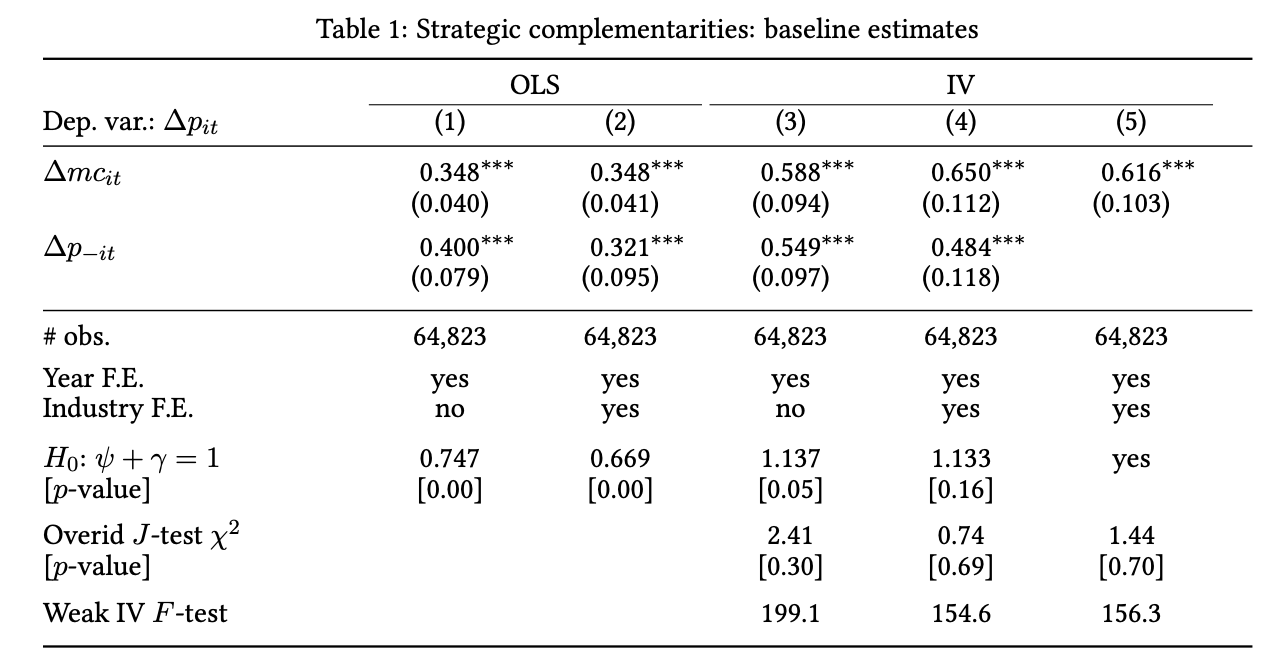
\includegraphics[scale=0.45]{FiguresTables/aik}
\end{figure}
Source: Amiti, Itskhoki, Konings (2019). Pass-through of 0.64
\end{frame}



\begin{frame}{Evidence?}
\begin{figure}
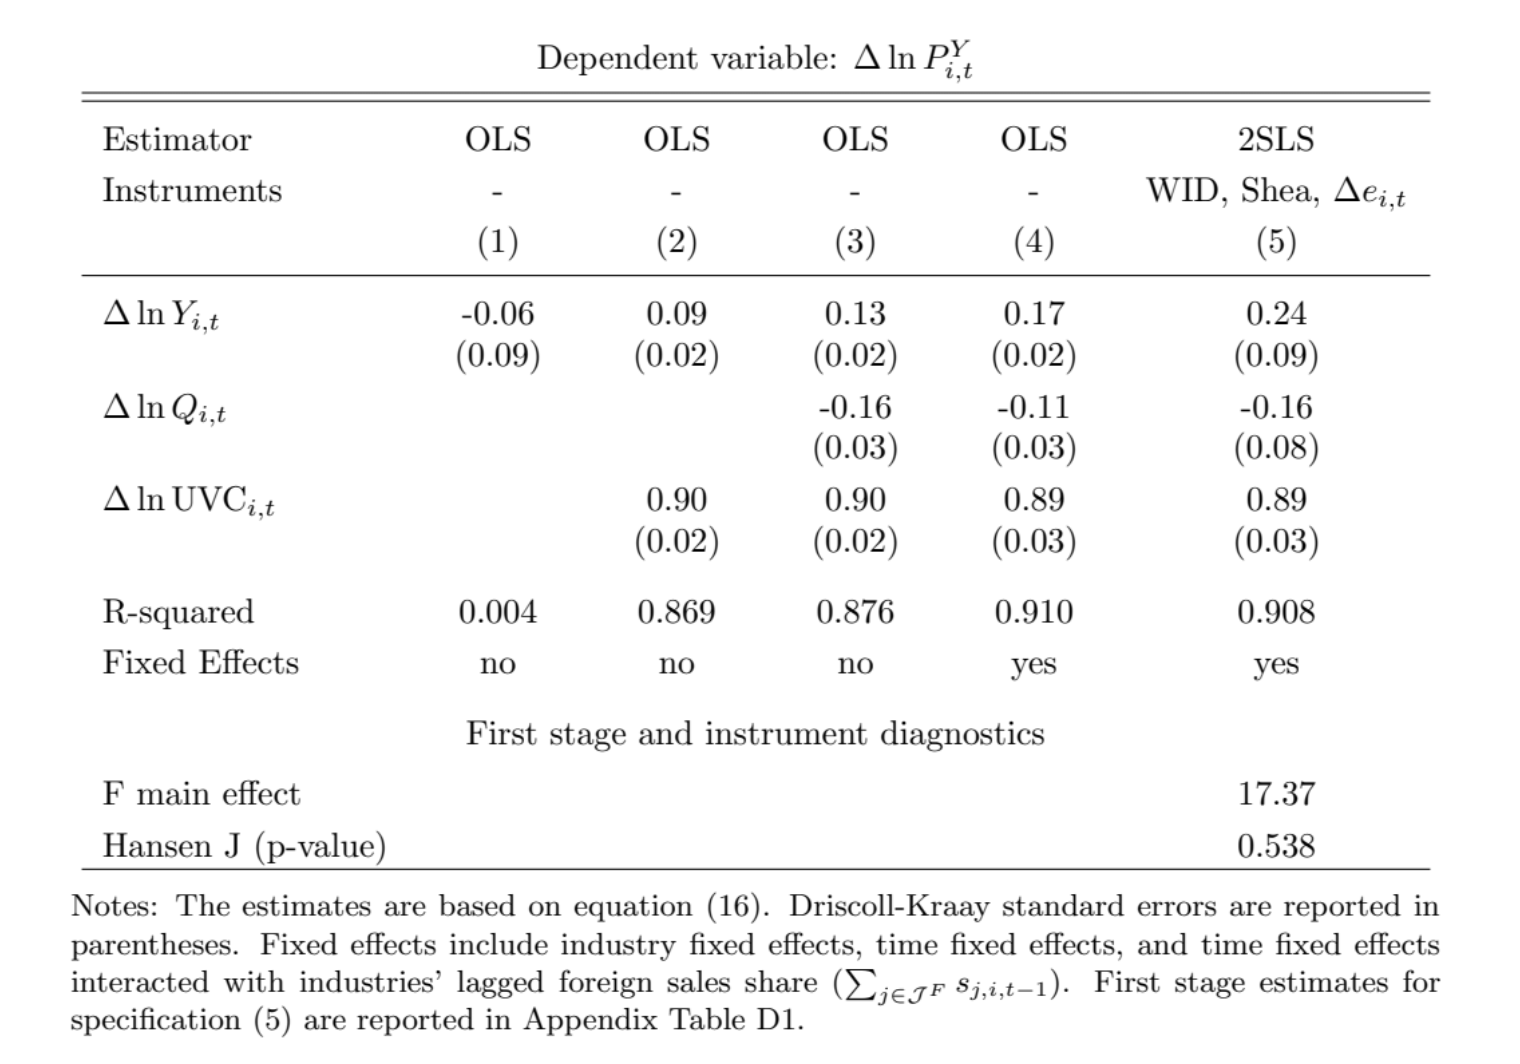
\includegraphics[scale=0.37]{FiguresTables/bpn}
\end{figure}
Source: Boehm, Pandalai-Nayar (2022). Marginal cost elasticity of 0.24.
\end{frame}


\begin{frame}{New back of the envelope}
\begin{itemize}
\item Don't put too much weight on these. Combines data sources, countries, methods, time aggregation.
\item Just want to illustrate the importance.
\item remember the slope $\kappa = \varphi \omega \Omega$
\item Using the textbook calibration: $\kappa \approx 0.2$.
\item Including real rigidities: $\kappa \approx 0.1 \times 0.64 \times 0.24 \approx 0.015$
\end{itemize}
\end{frame}
\end{document}




